\documentclass[11pt]{article}

\usepackage[a4paper, total={6.5in, 9.5in}]{geometry}
\usepackage{graphicx}
\usepackage{hyperref}
\usepackage{float}
\usepackage{amsmath}
\usepackage{tabularx}
\usepackage{booktabs}
\usepackage{multicol}
\usepackage{subcaption}
\usepackage{listings}
\usepackage{xcolor}
\usepackage{parskip}
\usepackage{titlesec}
\usepackage{microtype}
\usepackage{lscape}
\usepackage{tikz}

% Allow TeX extra stretch to handle long monospace identifiers
\emergencystretch=4em

% ── hyperref setup ──────────────────────────────────────────────────────────
\hypersetup{
  colorlinks=true,
  linkcolor=blue!60!black,
  urlcolor=blue!60!black,
  citecolor=blue!60!black
}

% ── code listing style ───────────────────────────────────────────────────────
\lstset{
  basicstyle=\ttfamily\footnotesize,
  frame=single,
  breaklines=true,
  keywordstyle=\color{blue!70!black},
  commentstyle=\color{gray},
  stringstyle=\color{red!70!black},
  showstringspaces=false,
  numbers=left,
  numberstyle=\tiny\color{gray},
  numbersep=6pt
}

% ── title ────────────────────────────────────────────────────────────────────
\title{
    \textbf{CUDA Special Course} \\
    \textbf{Project Report} \\[2.5em]
    
\includegraphics[width=0.18\textwidth]{../ProjectDescription/images/DTU.png}\\[2.5em]
    \textbf{License Plate Recognition on GPU using CUDA}
}

\author{
    \textbf{Dragos-Daniel Bonaparte}\\
    s256878@student.dtu.dk
}

\date{May 2026}

\begin{document}

\maketitle
\thispagestyle{empty}
\newpage
\setcounter{page}{1}
\tableofcontents
\newpage

\begin{abstract}
\noindent

This project ports a single-threaded OpenCV license-plate pipeline to CUDA C++. 
Every stage becomes a GPU kernel with no OpenCV dependency.
The goal of the project is to see how much speedup can be achieved by moving the computation to the GPU while retaining accuracy. The dataset contains 550 images, some which are easy to read and see, and some that are in bad lighting conditions or blurry. The pipeline achieves 932.6 img/s on an RTX 4070 Max-Q and 727.4 img/s on a GH200 — 6.50× and 5.07× 
over the CPU single-threaded baseline.
The surprising findings are that at 1280×720 the workload is clock-bound, not bandwidth- or SM-bound. 
The image fits in L2 and leaves most of the GH200's 132 SMs idle, so the smaller, higher-clocked GPU stays ≈1.29× ahead; the GH200 would most likely win at processing images with much larger resolutions. 
Against a hand-labelled ground truth, the GPU unfortunately reads plates less accurately than the OpenCV reference.


\end{abstract}

\newpage

% ============================================================
\section{Introduction}
\label{sec:intro}
% ============================================================

This is a license plate recognition pipeline written entirely in CUDA C++.
The pipeline is a hand-written port of an existing single-threaded OpenCV reference implementation~\cite{dahms_anpr}.

The project aimed to  parallelelize the project in CUDA, not to create a new recognition method: the vision algorithms (adaptive thresholding~\cite{bradley2007,gonzalez2018}, Otsu's method~\cite{otsu1979}, union-find connected-component labelling~\cite{stava2011,komura2015}, $k$-NN) are standard and are reimplemented as CUDA kernels.
Section~\ref{sec:results} reports both \emph{throughput} (the headline result) and \emph{recognition accuracy} against a hand-labelled ground truth, so despite speedup being an important metric, it is not the only consideration.
The key finding (Section~\ref{sec:discussion}) is that at 1280$\times$720 this workload is clock-bound: the smaller RTX 4070 outperforms the datacenter GH200, whose extra SMs and bandwidth are underutilized at these image resolutions.

All platforms process the same 550 images (1280$\times$720, \texttt{.ppm}) in the same sorted order; the experimental setup is detailed in Section~\ref{sec:setup}.

% ============================================================
\section{Pipeline Overview}
\label{sec:implemented}
% ============================================================

The pipeline is built from the following stages, every one a hand-written CUDA kernel validated against the CPU reference:

\begin{itemize}
  \item Background loader thread plus a 4-slot ping-pong upload pipeline (Section~\ref{sec:pingpong}).
  \item Scene preprocessing: eight kernels, BGR to a binary threshold image (Section~\ref{sec:preprocessing}).
  \item Connected-component labelling with a cooperative propagation kernel, then blob filtering (Section~\ref{sec:ccl}).
  \item Character grouping on the CPU (distance, angle, height similarity; Section~\ref{sec:platelocal}).
  \item Batched warp-crop: all plate candidates rectified in one kernel launch (Section~\ref{sec:platelocal}).
  \item Per-plate recognition: preprocess, resize, Otsu threshold, CCL, then $k$=1 KNN (Section~\ref{sec:charrec}, Listings~\ref{lst:otsu} and~\ref{lst:knn}).
  \item Pre-allocated GPU and pinned-host memory; no \texttt{cudaMalloc} in the scene loop (Section~\ref{sec:workspace}).
  \item End-to-end benchmarking with CSV output (Section~\ref{sec:results}).
\end{itemize}

% ============================================================
\section{System Architecture}
\label{sec:arch}
% ============================================================

Figure~\ref{fig:classdiagram} shows the module structure.
\texttt{PipelineContext} owns all GPU and pinned-host memory.
It allocates four \texttt{SceneBuffer} slots and one \texttt{PlateBuffer} per plate slot.
No \texttt{cudaMalloc} or \texttt{cudaFree} runs during the processing loop.

\begin{figure}[H]
  \centering
  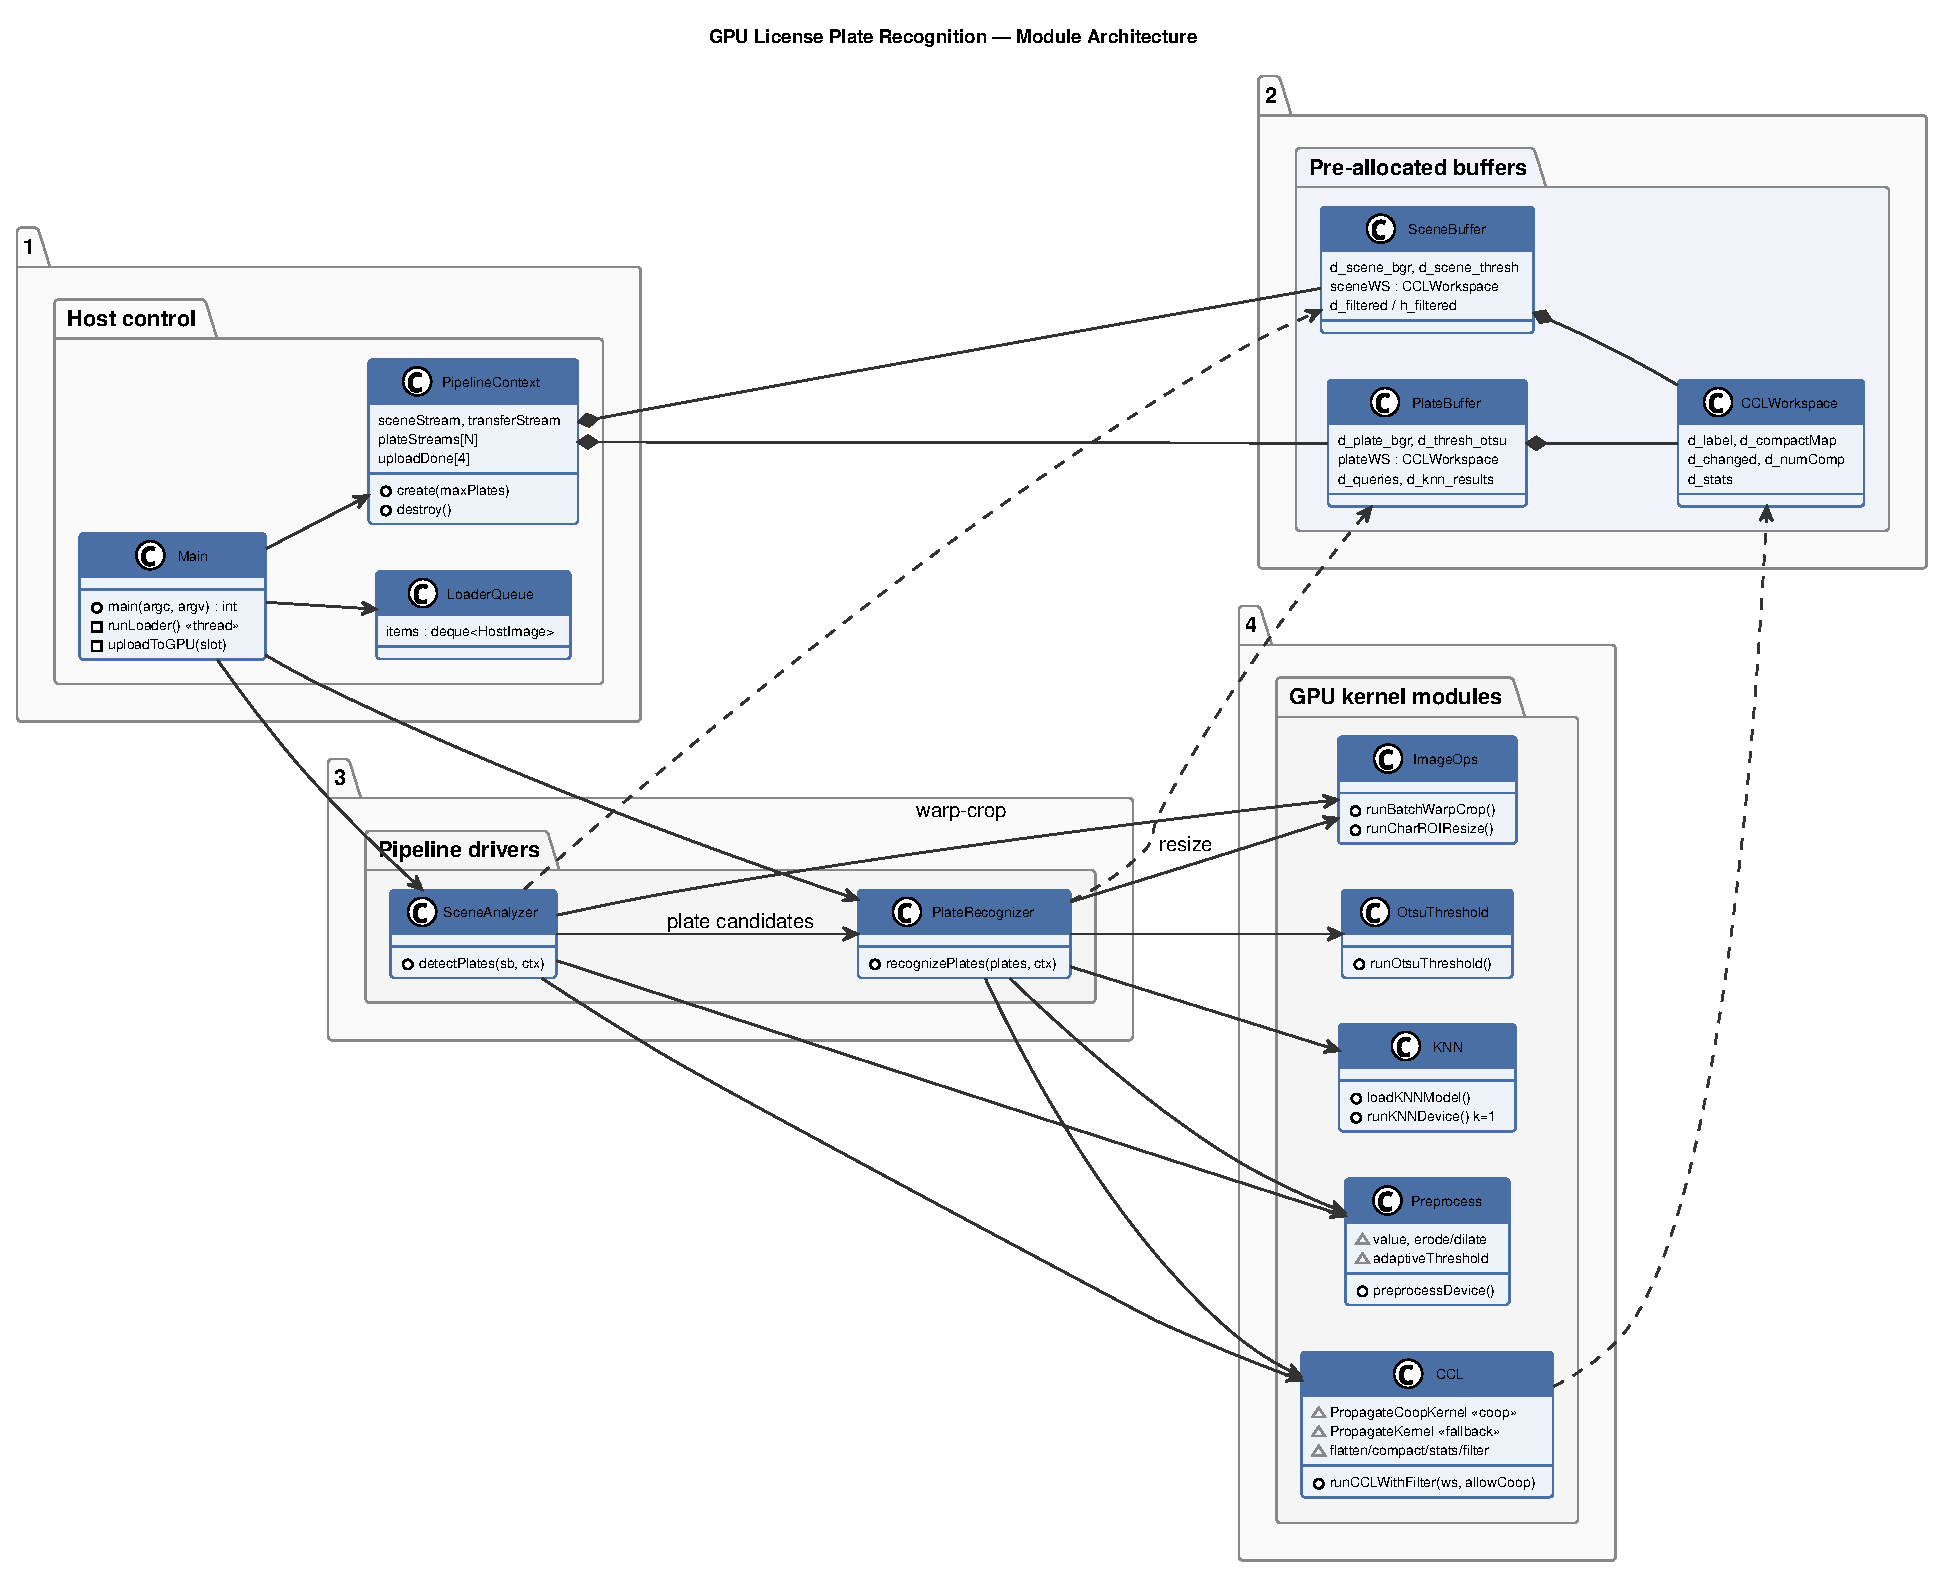
\includegraphics[width=\textwidth]{figures/classdiagram.pdf}
  \caption{Module architecture, grouped in four layers: host control, pre-allocated buffers,
           pipeline drivers, and GPU kernel modules. Diamonds denote composition; the bold
           arrow is the scene-to-plate handoff. Each \texttt{CCLWorkspace} is pre-allocated
           inside its \texttt{SceneBuffer} or \texttt{PlateBuffer}.}
  \label{fig:classdiagram}
\end{figure}

Three CUDA streams are used:
\begin{itemize}
  \item \texttt{sceneStream} -- scene kernels (preprocess, CCL, warp-crop).
  \item \texttt{transferStream} -- async H$\to$D uploads, decoupled from compute.
  \item \texttt{plateStreams[N]} -- one per plate slot; Wave~1 (CCL) and Wave~2 (KNN) run all $N$ in parallel.
\end{itemize}
The scene stream is gated by four \texttt{uploadDone} events, one per scene slot (\texttt{NUM\_SCENE\_SLOTS = 4}, the ping-pong depth of Section~\ref{sec:pingpong}).
Each event is recorded on \texttt{transferStream} once a slot's async upload completes; \texttt{sceneStream} then blocks on it with \texttt{cudaStreamWaitEvent} before reading that slot, so a kernel never touches a frame whose H$\to$D copy is still in flight.
This event handshake is the synchronisation half of the ping-pong pipeline detailed in Section~\ref{sec:pingpong}.

% ============================================================
\section{Pipeline Implementation}
\label{sec:pipeline}
% ============================================================

Figure~\ref{fig:activity} traces one image through the pipeline.

\begin{figure}[H]
  \centering
  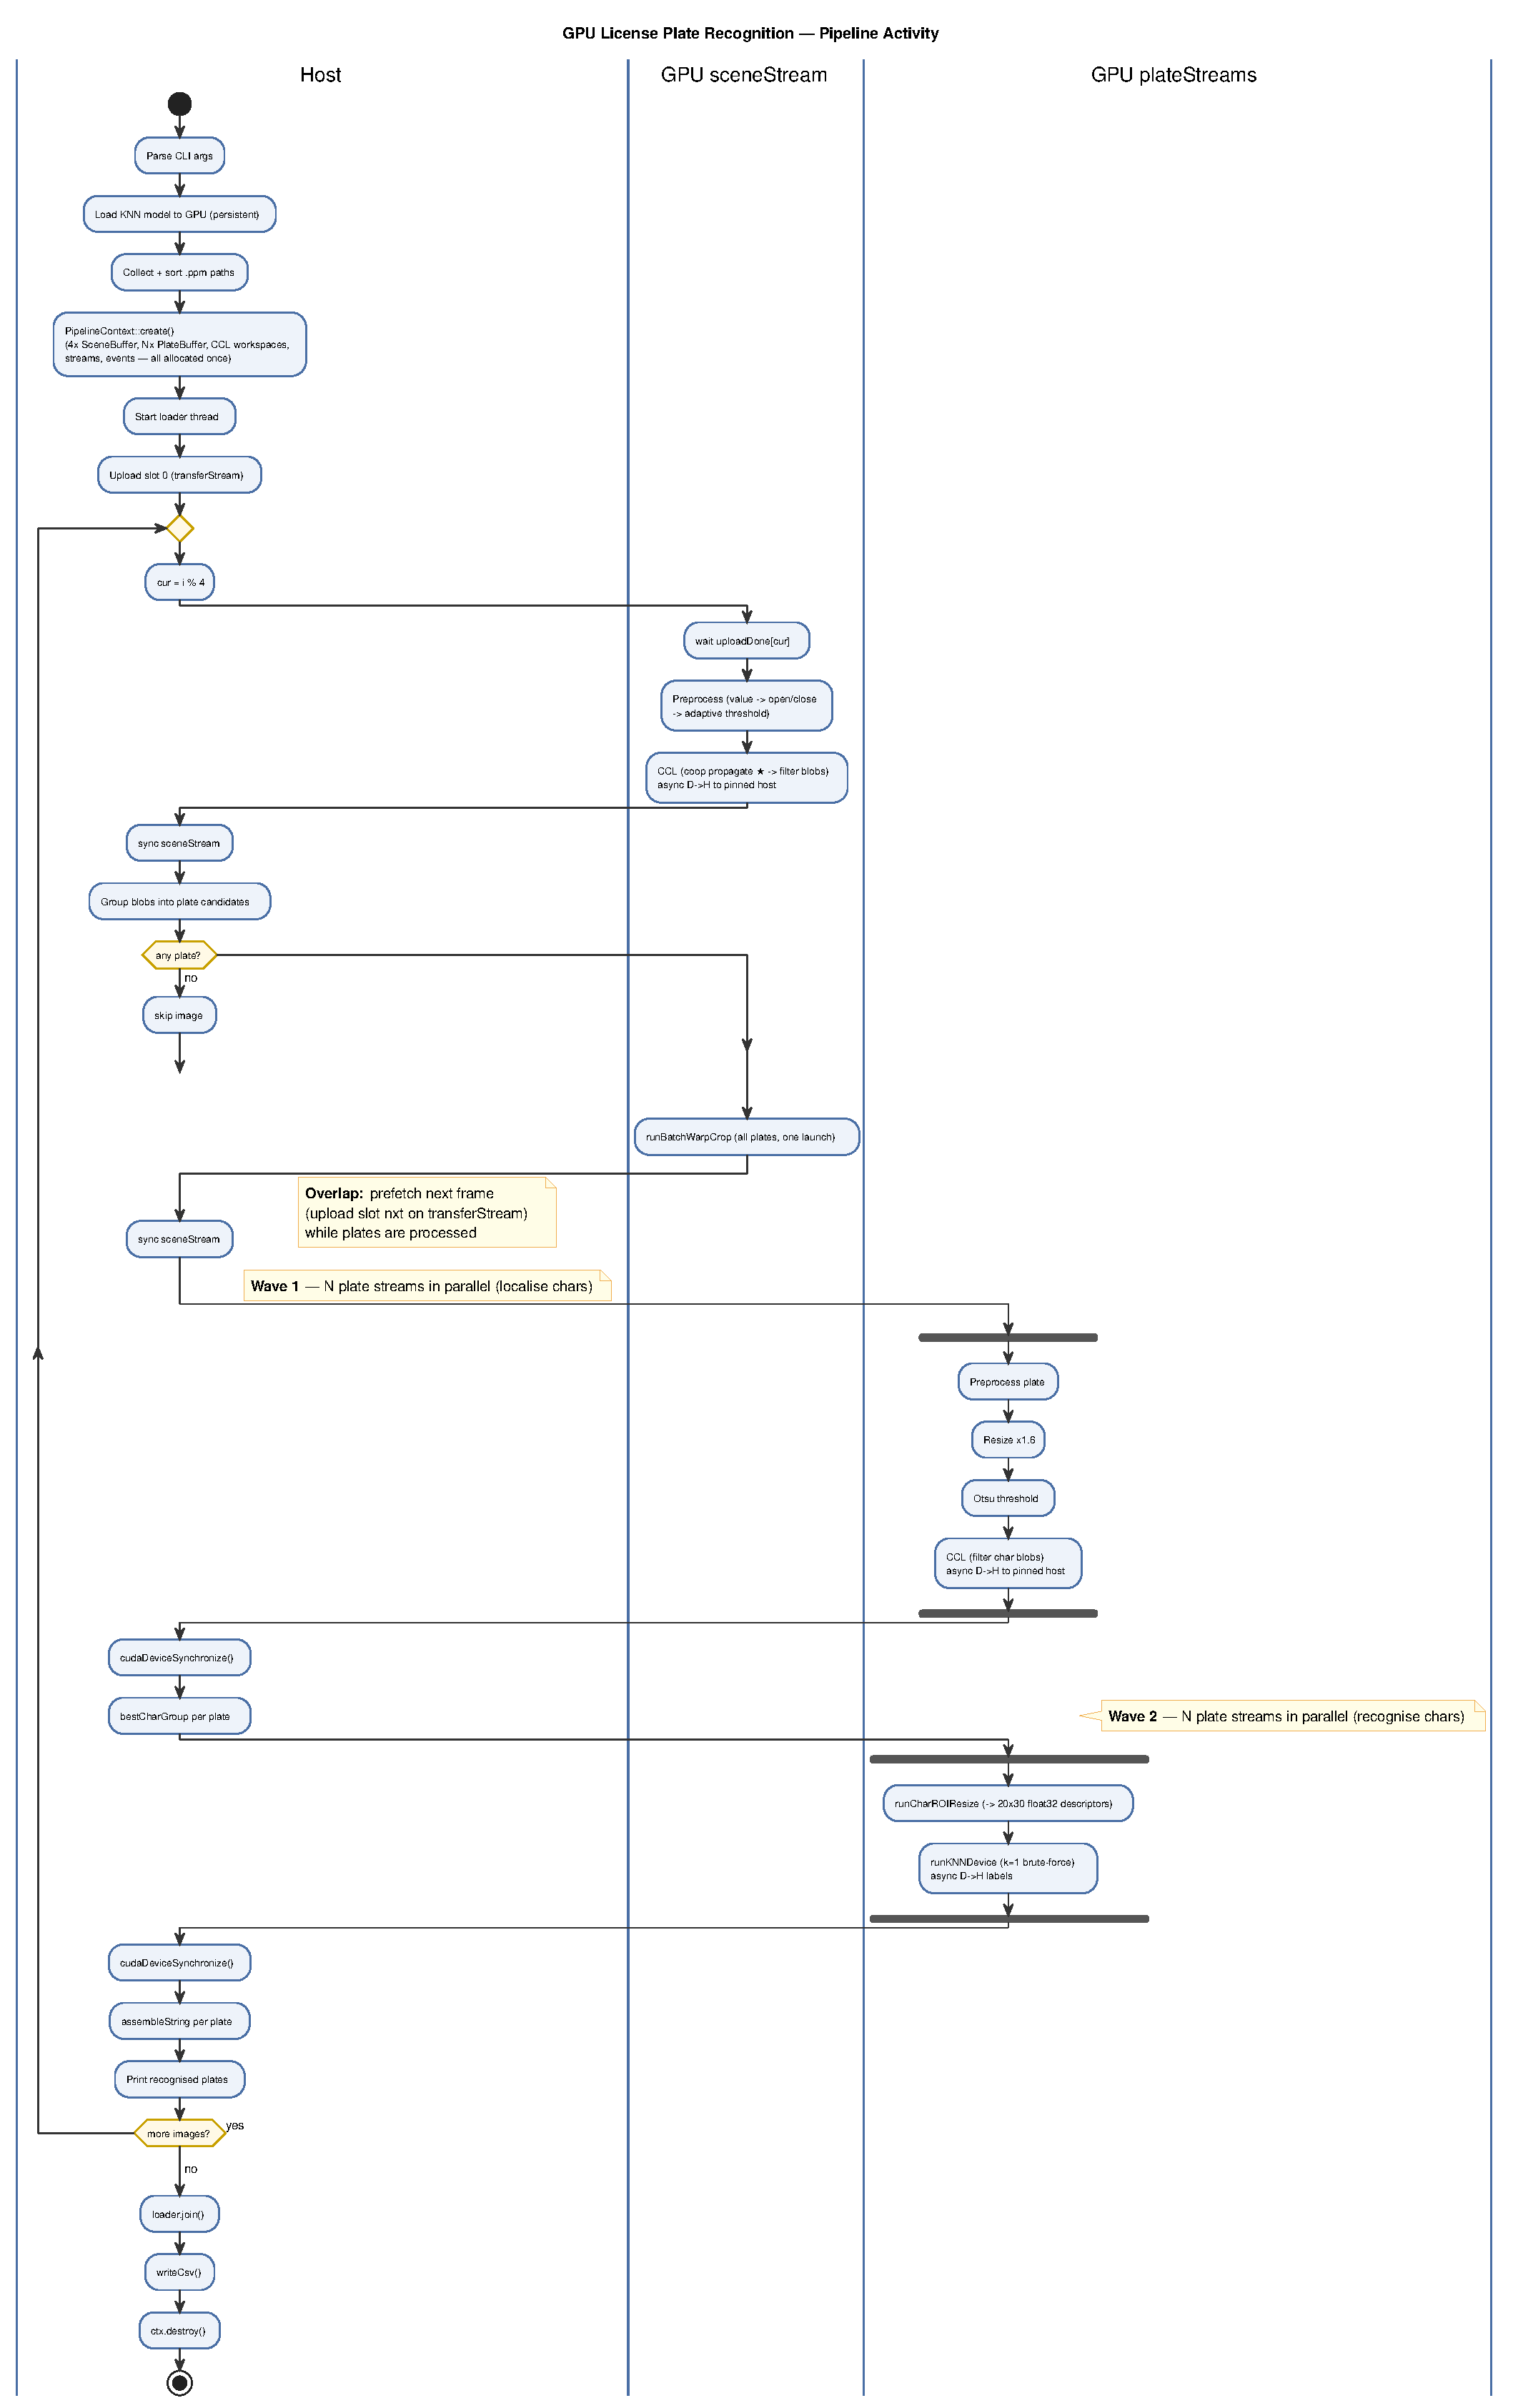
\includegraphics[height=0.92\textheight,keepaspectratio]{figures/activity.pdf}
  \caption{End-to-end pipeline. The Host lane drives CPU logic and sync points.
           The scene stream runs as one vertical pass. Wave~1 and Wave~2 each launch
           $N$ plate streams in parallel, separated by a device sync.}
  \label{fig:activity}
\end{figure}

The pipeline runs in two stages.
The \emph{scene stage} turns the full frame into character-sized blobs: preprocess, connected-component labelling (CCL), then group blobs into plate candidates.
The \emph{plate stage} processes each candidate on its own: rectify, threshold, a second CCL to split out characters, then KNN to read them.

\subsection{Preprocessing}
\label{sec:preprocessing}

Eight kernels run in sequence on the scene stream, mirroring the OpenCV reference's preprocessing.
They all operate on the \emph{value channel} --- the brightness (V) channel of the frame, where the bright/dark contrast of plate characters is strongest:

\begin{enumerate}
  \item \textbf{Value extraction} --- pull the brightness channel out of the BGR frame.
  \item \textbf{Opening} (erode then dilate, two kernels) --- \emph{erode} shrinks bright regions and \emph{dilate} grows them back; doing erode-then-dilate removes small bright specks (noise) while leaving larger shapes intact.
  \item \textbf{Closing} (dilate then erode, two kernels) --- the opposite order, which fills in small dark gaps inside bright regions.
  \item \textbf{Contrast maximisation} --- combine the opened and closed images to widen the gap between light and dark, so characters stand out from the background.
  \item \textbf{Gaussian blur} --- lightly smooth the result to suppress leftover pixel noise before thresholding.
  \item \textbf{Adaptive threshold} --- the final and heaviest kernel, which converts the grey image into a pure black-and-white (binary) image, \texttt{d\_scene\_thresh}.
\end{enumerate}

The adaptive threshold decides black-or-white per pixel by comparing each pixel to a Gaussian-weighted average of its \emph{local} neighbourhood, rather than to one global cut-off.
Using a local average means a bright patch of road and a shadowed patch are each judged against their own surroundings, so uneven lighting across the scene does not wash out the characters.

\subsection{CCL}
\label{sec:ccl}

Six kernels run in order:
\begin{enumerate}
  \item Init -- each foreground pixel gets its own label.
  \item Propagate -- iterative union-find with \texttt{atomicMin}; convergence is checked via \texttt{grid.sync()} in the cooperative variant (Section~\ref{sec:coop}).
  \item Flatten -- path-compress all labels to their roots.
  \item Compact -- assign dense component IDs via \texttt{atomicAdd}.
  \item Stats -- per-component bounding box and pixel count.
  \item Filter -- keep blobs within character bounds (area $>$ 80, $w > 2$, $h \ge 8$, $0.25 \le w/h \le 1.0$).
\end{enumerate}
The blobs that remain are copied asynchronously to pinned host memory on the same stream.

The core is the propagate kernel: every foreground pixel unions its label with its four neighbours, keeping the smallest root.
\texttt{atomicMin} makes the merge race-free, and \texttt{d\_changed} flags that another pass is needed.

\subsection{Plate localisation}
\label{sec:platelocal}

After the scene sync, \texttt{blobsToChars} and \texttt{groupChars} cluster character blobs by distance, angle, and height.
\texttt{runBatchWarpCrop} then crops and rectifies all plate candidates in one kernel launch.

\subsection{Character recognition}
\label{sec:charrec}

Each plate crop is preprocessed, resized $\times$1.6, and Otsu-thresholded.
Otsu picks a per-plate threshold from the intensity histogram, adapting to each plate's own contrast (Listing~\ref{lst:otsu}).

\begin{lstlisting}[caption={Otsu threshold: GPU histogram, CPU threshold search, GPU apply (\texttt{src/device/OtsuThreshold.cu}).},label={lst:otsu}]
# GPU: count how many pixels have each brightness 0..255 (a histogram)
each thread adds its pixels into a shared 256-bin histogram (atomicAdd),
then adds that block's histogram into the global one (atomicAdd)

# CPU: try every brightness cut-off, keep the one that splits best
for cutoff in 0..255:
    fracDark   = fraction of pixels darker than cutoff
    fracLight  = fraction of pixels brighter than cutoff
    meanDark   = average brightness of the dark pixels
    meanLight  = average brightness of the light pixels
    score[cutoff] = fracDark * fracLight * (meanDark - meanLight)^2
bestCutoff = the cutoff with the highest score   # groups most separated

# GPU: pixel >= bestCutoff ? white (255) : black (0)
\end{lstlisting}

CCL then extracts the characters.
Each is resized to a 20$\times$30 descriptor (600 float32 features) and classified by KNN (Listing~\ref{lst:knn}): one block per character, each thread owns one of the 180 training samples, and a shared-memory arg-min reduction picks the nearest.
\begin{lstlisting}[caption={KNN classify: one block per character, $k$=1 (\texttt{src/device/KNN.cu}).},label={lst:knn}]
each block = one query character; each thread = one of 180 samples
load the 600-feature query into shared memory; syncthreads()
dist[tid] = sum over 600 features of (query[i] - sample[tid][i])^2   # squared L2
syncthreads()
parallel arg-min reduction over dist[]  ->  nearest sample
thread 0: result = label[nearest]                                   # k = 1
\end{lstlisting}

% ============================================================
\section{Performance Optimisations}
\label{sec:opts}
% ============================================================

Before optimizations the RTX 4070 reached $\approx$700\,img/s and the GH200 reached $\approx$620\,img/s (both at \texttt{--max-plates 8}).
Three changes have raised those to 932.6 and 727.4\,img/s.

\subsection{Pre-allocated CCL workspaces}
\label{sec:workspace}

The original \texttt{runCCLWithFilter} ran five \texttt{cudaMalloc} calls on every frame and every plate crop, then freed them.
This was deliberate: \texttt{allocWorkspace(width\,$\times$\,height)} sized the workspace to each image exactly, so the program accepted any image size without knowing the dimensions in advance.
At 700\,img/s with eight plate slots that is $700 \times 9 \times 5 \approx 31\,500$ allocator calls per second.

Each \texttt{SceneBuffer} and \texttt{PlateBuffer} now owns a persistent \texttt{CCLWorkspace} (five device buffers, allocated once at startup).
A \texttt{cudaMemsetAsync} resets the counters between frames.
The trade-off is the lost flexibility: the workspaces are sized once to fixed maxima using a python script, (\texttt{SCENE\_W$\times$SCENE\_H} for scenes, \texttt{MAX\_PLATE\_THRESH\_W$\times$MAX\_PLATE\_THRESH\_H} for plates), which is why the input is now fixed at 1280$\times$720.

\begin{table}[H]
\centering
\begin{tabular}{lcc}
\toprule
 & Before & After \\
\midrule
\texttt{cudaMalloc}/\texttt{cudaFree} per image & $\approx$90 & 0 \\
CCL workspace lifetime & per-call & persistent \\
\bottomrule
\end{tabular}
\caption{CCL workspace allocation before and after.}
\label{tab:workspace}
\end{table}

\subsection{Cooperative propagation kernel}
\label{sec:coop}

The original convergence loop did one host round-trip per iteration: \texttt{cudaStreamSynchronize}, then two blocking \texttt{cudaMemcpy} calls (reset the flag H$\to$D, read it back D$\to$H).
Each round-trip costs $\approx$30\,$\mu$s; 20--50 iterations per scene added 0.6--1.5\,ms per image.
On the GH200 the kernels are faster, so the fixed round-trip cost is a larger share of total time, which is part of why the GH200 was initially slower (Section~\ref{sec:discussion}).

The replacement, \texttt{cclPropagateCoopKernel}, is launched with \texttt{cudaLaunchCooperativeKernel}.
All thread blocks are resident at once, which enables \texttt{grid.sync()} inside the kernel which is a barrier that waits for \emph{every} thread in \emph{every} block across the whole grid, not just the threads in one block.
Three grid barriers per iteration replace the host round-trips:

\begin{lstlisting}[language=C++, caption={Three-sync convergence pattern.}]
for (int iter = 0; iter < maxIter; iter++) {
    if (tid == 0) *d_changed = 0;
    grid.sync();                          // sync 1: all threads see reset

    /* propagation: atomicMin + atomicOr(d_changed, 1) */

    grid.sync();                          // sync 2: all writes visible

    bool converged = (*d_changed == 0);   // cache before sync 3

    grid.sync();                          // sync 3: prevent race on next reset
    if (converged) break;
}
\end{lstlisting}

Sync 3 is required.
Without it the fastest block races ahead and resets \texttt{d\_changed} before slower blocks have read it, so they break early and deadlock at the next \texttt{grid.sync()}.

\subsection{4-slot ping-pong pipeline}
\label{sec:pingpong}

A background loader thread feeds images into a bounded queue (capacity 3).
Uploads run on \texttt{transferStream}; a \texttt{cudaStreamWaitEvent} on \texttt{sceneStream} delays kernel launch until the current slot's upload finishes.
This hides the H$\to$D transfer behind compute across four scene slots.

Figure~\ref{fig:pipeline_overlap} shows the steady state.
Each frame (one colour) flows diagonally down the four lanes: load, then upload, then scene compute, then plate compute.
At any instant four different frames occupy the four lanes, so the H$\to$D upload of one frame runs while the GPU computes another.

\begin{figure}[H]
\centering
\resizebox{\textwidth}{!}{%
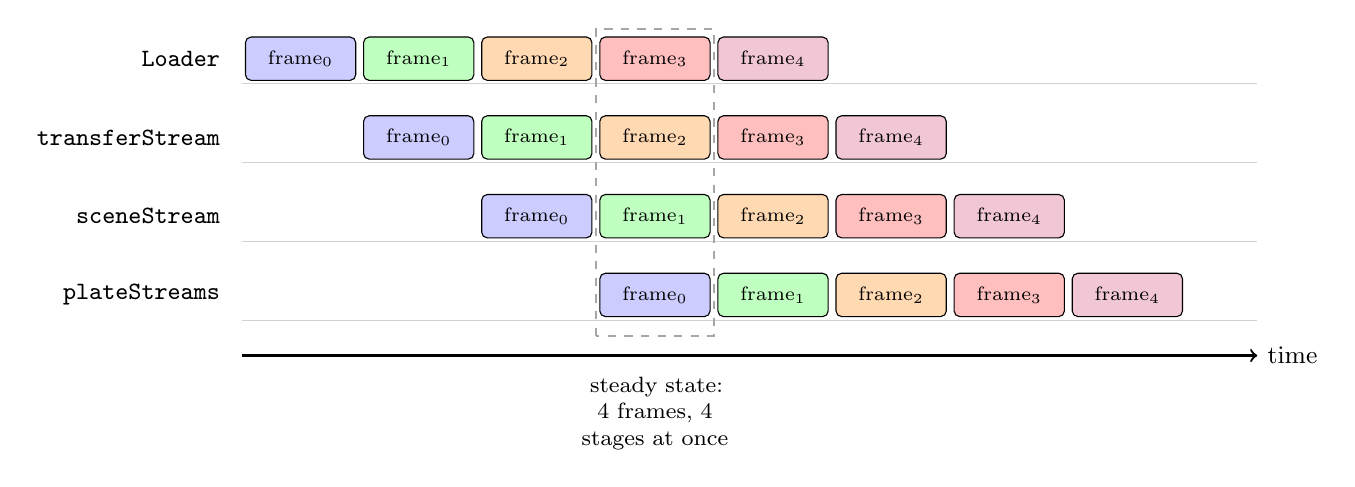
\begin{tikzpicture}[x=1.5cm,y=1.0cm,
  lane/.style={font=\small\ttfamily},
  blk/.style={draw,rounded corners=2pt,minimum width=1.4cm,
              minimum height=0.55cm,inner sep=1pt,font=\scriptsize}]

  % lane baselines + labels (top-to-bottom = data dependency order)
  \foreach \name/\yy in {Loader/3, transferStream/2, sceneStream/1, plateStreams/0} {
    \node[lane,anchor=east] at (-0.1,\yy+0.32) {\name};
    \draw[gray!35] (0,\yy) -- (8.6,\yy);
  }

  % steady-state highlight: one time column, four frames in four stages
  \draw[dashed,thick,gray!70] (3,-0.2) rectangle (4,3.7);

  % each frame k: load@k, upload@k+1, scene@k+2, plate@k+3
  \foreach \k/\col in {0/blue!20, 1/green!25, 2/orange!30, 3/red!25, 4/purple!22} {
    \node[blk,fill=\col] at ({\k+0.5},3.32) {frame$_{\k}$};
    \node[blk,fill=\col] at ({\k+1.5},2.32) {frame$_{\k}$};
    \node[blk,fill=\col] at ({\k+2.5},1.32) {frame$_{\k}$};
    \node[blk,fill=\col] at ({\k+3.5},0.32) {frame$_{\k}$};
  }

  % time axis
  \draw[->,thick] (0,-0.45) -- (8.6,-0.45) node[anchor=west,font=\small]{time};
  \node[font=\footnotesize,anchor=north,text width=3.2cm,align=center]
        at (3.5,-0.6) {steady state:\\4 frames, 4 stages at once};

\end{tikzpicture}%
}
\caption{4-slot ping-pong in steady state. Time runs left to right; lanes are stacked in
         dependency order. Each frame (one colour) steps diagonally: load $\to$ upload
         $\to$ scene $\to$ plate. The dashed column shows that at one instant frame$_3$ loads,
         frame$_2$ uploads, frame$_1$ runs scene kernels, and frame$_0$ runs plate kernels, so
         transfer is fully hidden behind compute.}
\label{fig:pipeline_overlap}
\end{figure}

% ============================================================
\section{Experimental Setup}
\label{sec:setup}
% ============================================================

\subsection{Platforms}

\begin{table}[H]
\centering
\begin{tabular}{p{3.2cm}p{2.8cm}p{2cm}p{4cm}}
\toprule
Platform & GPU & VRAM & Notes \\
\midrule
CPU baseline          & ---            & ---          & AMD Ryzen 7 7745HX, single-threaded OpenCV \\
NVIDIA RTX 4070 Max-Q & Ada Lovelace   & 8\,GB GDDR6  & 36 SMs, 3105\,MHz max, PCIe Gen4 \\
NVIDIA GH200          & Hopper (H100)  & 96\,GB HBM3e & 132 SMs, 1980\,MHz max, NVLink-C2C \\
\bottomrule
\end{tabular}
\caption{Evaluation platforms.}
\label{tab:platforms}
\end{table}

The CPU baseline runs single-threaded on an AMD Ryzen 7 7745HX (8 cores, 16 threads, up to 5.15\,GHz boost, 32\,MB L3).

\subsection{Dataset and metrics}

All runs use the same 550 images, some of which are easy to read and see, and some that are in bad lighting conditions or blurry.
The CPU reads the images in the \texttt{.jpg} format, while the GPU reads them in the \texttt{.ppm} format.
The frames are processed in the same order, so frame $i$ is identical across platforms.
Wall-clock time covers the full loop, from the first upload to the final \texttt{cudaDeviceSynchronize}.
The primary metric is throughput (img/s); recognition quality is reported separately in Section~\ref{sec:accuracy} against a hand-labelled ground truth of 119 frames.

\subsection{Compilation and measurement}

The binary is compiled with \texttt{-O3 -arch=sm\_89} for the RTX~4070 and \texttt{-arch=sm\_90} for the GH200; cooperative launch requires \texttt{-rdc=true}.
Each configuration was run five times back-to-back and the steady-state run reported.
The first 2 runs are discarded and considered warm-up.

% ============================================================
\section{Results}
\label{sec:results}
% ============================================================

\subsection{Throughput}

\begin{table}[H]
\centering
\begin{tabular}{lrr}
\toprule
Platform & Throughput (img/s) & Speedup vs CPU \\
\midrule
CPU baseline   & 143.4 & 1.00$\times$ \\
RTX 4070 Max-Q & 932.6 & 6.50$\times$ \\
GH200          & 727.4 & 5.07$\times$ \\
\bottomrule
\end{tabular}
\caption{Final benchmark results on the 550-image set (\texttt{--max-plates 8}). Speedups are relative to the single-threaded CPU baseline (Section~\ref{sec:setup}).}
\label{tab:crossplatform}
\end{table}

The CUDA pipeline reaches 6.50$\times$ the single-threaded OpenCV baseline on the RTX 4070 and 5.07$\times$ on the GH200.
Section~\ref{sec:discussion} will explain the assumptions of why the RTX4070 is faster than the GH200.

\subsection{Recognition accuracy}
\label{sec:accuracy}

Throughput only matters if the pipeline still reads the right plates, so 119 frames spanning the sequence were hand-labelled to form a ground truth.
For each labelled frame a pipeline is scored on its best printed candidate.
Three quantities are reported (Table~\ref{tab:accuracy}): the \emph{detection rate} (fraction of ground-truth frames for which at least one plate string was emitted), the \emph{exact-match rate} (best candidate equals the label character-for-character), and \emph{character similarity}

\begin{table}[H]
\centering
\small
\begin{tabular}{lrr}
\toprule
Metric (over 119 ground-truth frames) & CPU (OpenCV) & GPU (CUDA) \\
\midrule
Detection rate (\%)        & 68.9 & 51.3 \\
Exact plate match (\%)     &  7.6 &  2.5 \\
Character similarity (\%)  & 33.6 & 23.9 \\
\bottomrule
\end{tabular}
\normalsize
\caption{Recognition accuracy against hand-labelled ground truth.}
\label{tab:accuracy}
\end{table}

Two things stand out. 
First, accuracy is low on both pipelines. Perhaps the dataset chosen as benchmark is too difficult for both algorithms given that even the OpenCV reference rarely gets a plate exactly right. Second, the GPU is clearly doing worse than the OpenCV baseline. 
It finds a plate in 51.3\% of labelled frames, while the CPU finds one in 68.9\%, and it matches the full plate exactly far less often. 
The handwritten CUDA detection, thresholding, and brute-force KNN are simpler than OpenCV's versions, and they lose accuracy on the hardest frames. When both pipelines do return a plate, they agree exactly only 5.0\% of the time and reach 51.4\% character similarity. 
Section~\ref{sec:correctness} looks at a run of consecutive frames one by one.

\subsection{Max-plates sweep}
\label{sec:sweep}

\texttt{--max-plates} sets the number of pre-allocated plate slots and parallel plate streams: a low value runs fewer plate streams (higher throughput) but caps how many plates per frame can be recognised (lower recall).
Table~\ref{tab:sweep} sweeps it on both GPUs.
\texttt{--max-plates} 1 is the fastest setting (1060\,img/s on the RTX 4070) but only finds 423 plates across the set; \texttt{--max-plates} 8 gives up $\approx$12\% throughput to find 927 plates, and detection does not increase much afterwards.
The headline results (Table~\ref{tab:crossplatform}) use \texttt{--max-plates} 8 because the program is meant ultimately to detect license plates, not necessarly peak throughput, and is what makes the accuracy in Table~\ref{tab:accuracy} meaningful.

\begin{table}[H]
\centering
\small
\begin{tabular}{rrrrr}
\toprule
 & \multicolumn{2}{c}{\textbf{RTX 4070 Max-Q}} & \multicolumn{2}{c}{\textbf{GH200}} \\
\cmidrule(lr){2-3} \cmidrule(lr){4-5}
\texttt{max-plates} & img/s & Plates & img/s & Plates \\
\midrule
 1 & 1060.2 & 423 &  813.2 & 423 \\
 2 &  991.4 & 658 &  769.9 & 654 \\
 4 &  948.6 & 863 &  734.2 & 849 \\
 8 &  932.6 & 927 &  727.4 & 903 \\
16 &  934.8 & 931 &  725.0 & 903 \\
32 &  928.6 & 928 &  722.4 & 899 \\
\midrule
RTX/GH200 ratio & \multicolumn{2}{c}{$\approx$1.29$\times$ (constant)} & & \\
\bottomrule
\end{tabular}
\normalsize
\caption{Throughput sweep over \texttt{--max-plates}, both platforms.}
\label{tab:sweep}
\end{table}

\begin{itemize}
  \item The RTX/GH200 ratio is $\approx$1.29$\times$ at every value. This is a structural gap, not load-dependent.
  \item Throughput drops from $N$=1 to $N$=4 ($-$10\%), then flattens ($-$0.9\% from 4 to 8). Scene work (adaptive threshold + CCL) dominates; plate streams add little once the scene is done.
  \item Detection saturates at $N$=8: $N$=8 and $N$=16 find the same number of plates, so $N$=8 is the best operating point.
  \item The GH200 degrades more gracefully ($-$10.5\% from 1 to 8 vs $-$12.0\% on the RTX 4070) because its 132 SMs absorb parallel plate streams better.
\end{itemize}

% ============================================================
\section{Profiling Analysis}
\label{sec:profiling}
% ============================================================

Both GPUs were profiled with \texttt{nsys profile --trace=cuda,nvtx} over the same 550 images.

\subsection{CUDA API time}

\begin{table}[H]
\centering
\small
\begin{tabular}{lrrrr}
\toprule
 & \multicolumn{2}{c}{\textbf{RTX 4070}} & \multicolumn{2}{c}{\textbf{GH200}} \\
\cmidrule(lr){2-3} \cmidrule(lr){4-5}
API call & \% & Calls & \% & Calls \\
\midrule
\texttt{cudaStreamSynchronize}       & 39.5 & 2\,948  & 59.9 & 2\,904 \\
\texttt{cudaMemcpyAsync}             & 21.0 & 5\,546  &  6.3 & 5\,458 \\
\texttt{cudaMalloc}                  & 12.9 & 1\,158  & 13.7 & 1\,136 \\
\texttt{cudaLaunchKernel}            &  9.9 & 28\,207 &  6.9 & 27\,728 \\
\texttt{cudaMemcpy} (blocking)       &  5.1 & 5\,504  &  7.1 & 5\,382 \\
\texttt{cudaDeviceSynchronize}       &  2.3 &    850  &  3.4 &    838 \\
\texttt{cudaLaunchCooperativeKernel} &  0.2 &    550  &  0.2 &    550 \\
\bottomrule
\end{tabular}
\normalsize
\caption{CUDA API summary, both platforms (550 images).}
\label{tab:api_sum}
\end{table}

\texttt{cudaStreamSynchronize} is the most time-consuming API call on both platforms, but more so on the GH200 (59.9\% vs 39.5\%).
It comes from two explicit syncs per image in \texttt{SceneAnalyzer} plus one per plate in the plate CCL loop.
The GH200 pays a larger share because its kernels finish faster while its host round-trips do not, so the fixed sync cost is a bigger fraction of total time (Section~\ref{sec:discussion}).
\texttt{cudaMalloc} costs $\approx$13\% on both ($\approx$1150 calls) from kernels which still allocate per call.
The RTX spends more of its API time in memory copies (PCIe); the GH200 spends more in stream syncs.
\texttt{cudaLaunchCooperativeKernel} costs only 0.2\% on both.

\subsection{GPU kernel time}

\begin{table}[H]
\centering
\small
\begin{tabular}{lrr}
\toprule
Kernel & RTX 4070 \% & GH200 \% \\
\midrule
\texttt{adaptiveThresholdKernel}    & 26.5 & 59.4 \\
\texttt{cclPropagateCoopKernel}     & 21.7 & 14.9 \\
\texttt{cclStatsKernel}             & 13.1 &  7.8 \\
\texttt{erodeKernel / dilateKernel} & 13.4 &  3.8 \\
\texttt{gaussianBlurKernel}         &  5.0 &  1.2 \\
\texttt{extractValueKernel}         &  4.3 &  1.4 \\
\texttt{cclPropagateKernel}         &  3.5 &  3.1 \\
\texttt{knnKernel}                  &  3.5 &  3.0 \\
Other                               &  9.0 &  5.4 \\
\bottomrule
\end{tabular}
\normalsize
\caption{GPU kernel time share, both platforms (550 images).}
\label{tab:kern_sum}
\end{table}

\texttt{adaptiveThresholdKernel} is the most expensive kernel on both, and far more expensive on the GH200 (59.4\% vs 26.5\%).
\texttt{cclPropagateCoopKernel} runs once per image (550 times) and is the scene CCL.
\texttt{cclPropagateKernel} is plate CCL ($\approx$2700 instances, $\approx$5 iterations/image): fast kernels, but bound by the host round-trip per iteration.
\texttt{knnKernel} costs $\approx$3\% on both; brute-force $k$=1 over 180 samples should not be a bottleneck.

% ============================================================
\section{Discussion}
\label{sec:discussion}
% ============================================================

\subsection{The GH200's early bottlenecks}

The GH200 first reached only $\approx$620\,img/s versus $\approx$700\,img/s on the RTX~4070, despite 3.7$\times$ more SMs and 13$\times$ more memory bandwidth.
Two bottlenecks that do not scale with SM count explain this:

\begin{enumerate}
  \item Allocator contention. The CUDA allocator is a global lock. The GH200's faster kernels drive a higher frame-rate attempt, so they hit the allocator more often per second and serialise harder.
  \item Host round-trip penalty. The CCL fallback loop costs $\approx$30\,$\mu$s per iteration regardless of SM count. The GH200 finishes each kernel iteration faster, so the fixed overhead is a larger fraction of per-frame time.
\end{enumerate}

Pre-allocated workspaces remove the allocator pressure.
The cooperative kernel removes the round-trips for scene CCL, which is the dominant CCL call.

\subsection{Comparing the two GPUs at this scale}

After the fixes the RTX~4070 leads by $\approx$1.29$\times$ at every configuration.
The raw SM clock ratio is $3105 / 1980 = 1.57\times$ (from \texttt{nvidia-smi}).
The observed gap (1.29$\times$) is narrower than the clock gap (1.57$\times$): the GH200 architecture recovers $\approx$18\%, but cannot close it at this image scale.

The GH200's advantages that do not help here:

\begin{enumerate}
  \item NVLink-C2C bandwidth (28$\times$ faster H$\to$D). The ping-pong pipeline already hides transfers. A 2.76\,MB frame takes 206\,$\mu$s on PCIe and 7\,$\mu$s on NVLink-C2C; both are shorter than the $\approx$1\,ms compute time, so neither platform is transfer-bound.
  \item HBM3e bandwidth (13$\times$ higher). The 0.9\,MB scene fits in both GPUs' L2 caches (RTX 4070: 36\,MB, GH200: 50\,MB). No DRAM transaction occurs in steady state, so the bandwidth gap is invisible.
  \item SM count (3.7$\times$ more). At 1280$\times$720 the cooperative CCL launches $132 \times 2 = 264$ blocks for 921\,600 pixels: about 13 pixels per thread. Most GH200 SMs sit idle; this workload is per-SM throughput, where clock speed wins.
\end{enumerate}

Table~\ref{tab:bandwidth} shows measured bandwidth and latency from \texttt{nvbandwidth v0.9}.

\begin{table}[H]
\centering
\begin{tabular}{lrrr}
\toprule
Metric & GH200 & RTX 4070 & Ratio \\
\midrule
H2D bandwidth, CE (GB/s)      & 380.1  & 13.4  & 28.4$\times$ GH200 \\
D2H bandwidth, CE (GB/s)      & 297.7  & 13.5  & 22.1$\times$ GH200 \\
Bidirectional H2D, CE (GB/s)  & 178.3  & 13.3  & 13.4$\times$ GH200 \\
Bidirectional D2H, CE (GB/s)  & 189.0  & 11.6  & 16.3$\times$ GH200 \\
CPU--GPU latency, SM (ns)     & 617.7  & 563.7 & 1.09$\times$ RTX faster \\
Device local copy (GB/s)      & 1462.4 & 112.7 & 13.0$\times$ GH200 \\
\bottomrule
\end{tabular}
\caption{Bandwidth and latency from \texttt{nvbandwidth v0.9} (GH200 NVLink-C2C vs RTX 4070 PCIe).}
\label{tab:bandwidth}
\end{table}

The GH200's CPU--GPU latency (617.7\,ns) is 9.5\% higher than the RTX 4070 (563.7\,ns).
The plate CCL fallback issues two latency-bound 4-byte \texttt{cudaMemcpy} calls per iteration; across 2690 iterations that adds $\approx$0.3\,ms.
NVLink-C2C does not reduce small-transfer latency below PCIe in these experiments.

The GH200's advantages only show with larger workloads.
At 4K the CCL and threshold kernels would launch $\approx$9$\times$ more blocks, the cooperative kernel could saturates all 132 SMs, and the 13$\times$ bandwidth advantage would be obvious.

\subsection{Correctness versus the CPU baseline}
\label{sec:correctness}

The aggregate accuracy in Section~\ref{sec:accuracy} is best understood frame by frame.
Table~\ref{tab:correctness} shows a consecutive sample (frames 453--468), a clearer close-up segment of the set where both pipelines do better than their averages, with the hand-labelled ground truth alongside.

\begin{table}[H]
\centering
\small
\begin{tabular}{rllll}
\toprule
Frame & Ground truth & CPU (OpenCV) & GPU (CUDA) & Note \\
\midrule
453 & MCLRNF1  & MCLRNF1  & N0LPNE1  & CPU exact \\
454 & ZOOMN65  & Z00MN65  & ---      & CPU O$\to$0; GPU miss \\
455 & HOR5SH1T & HUR5SH1T & HDH5SH1T & close \\
456 & FALLYOU  & FALLY9U  & EALLYBB  & both poor \\
457 & EZEY     & EZEY     & EZEY     & all exact \\
458 & NITESKY  & NITESIY  & N1TESKY  & close \\
459 & U8NTBAD  & U8NTBAD  & 68NTBAB  & CPU exact \\
460 & GAY247   & 0AY247   & 8AY247   & 1 char each \\
461 & LOLWATT  & L0LWATT  & WATT4    & CPU close; GPU partial \\
462 & RIPLS1   & RIPLS1   & PJPLS1   & CPU exact \\
463 & NICESKY  & 1N1CESY  & NT0ESKY  & both poor \\
464 & NVSBLE   & NVSBLE   & ---      & CPU exact; GPU miss \\
465 & NYSJ     & NYSJ     & NYSJ     & all exact \\
466 & ANBYOND  & ANBYOND  & ZNBYOYB  & CPU exact \\
467 & 1ZM961   & 1ZP961   & 1ZM961   & GPU exact \\
468 & PNYEXPS  & PNYEXPS  & PNYEIPS  & CPU exact \\
\bottomrule
\end{tabular}
\normalsize
\caption{Per-frame plate readings, ground truth vs CPU vs GPU (frames 453--468). Only the candidate closest to the ground truth is shown}
\label{tab:correctness}
\end{table}

The two pipelines localise and read the same plates on the same frames: several exact matches, and several more within a single character.
Despite rewriting the OpenCV stages by hand in CUDA, the behaviour is not exactly equivalent in every case, and the aggregate in Table~\ref{tab:accuracy} confirms the GPU is worse at detection.

\subsection{Other optimizations that could be explored}
\label{sec:future}

The profiling points to a few areas worth investigating further.
The adaptive-threshold kernel is the largest single cost (27--59\% of GPU time), so it is the first target for further kernel-level optimisation.
On the API side, \texttt{cudaMalloc} still costs $\approx$13\% (the plate warp-crop and char-resize paths allocate per call) and \texttt{cudaStreamSynchronize} takes the largest share (mostly the plate-CCL fallback loop and the per-plate Otsu histogram round-trip, Section~\ref{sec:charrec}), so both the remaining hot-path allocations and the per-iteration host syncs are clear next steps.
The high \texttt{cudaLaunchKernel} count ($\approx$28,000) and the repeated morphology passes also leave launch overhead on the table; the pipeline was split into many small, single-purpose kernels for readability, and fusing them would reduce it.
On the recognition side, the modest accuracy in Table~\ref{tab:accuracy} suggests the brute-force $k$=1 KNN and the simple blob filter are the limiting factors.

% ============================================================
\section{Conclusions}
\label{sec:conclusions}
% ============================================================

The project ported a single-threaded OpenCV license-plate pipeline into a full CUDA implementation with no vision library, reaching 932.6\,img/s on an RTX~4070 (6.50$\times$ the single-threaded baseline) and 727.4\,img/s on a GH200 (5.07$\times$).
Pre-allocated workspaces and a cooperative-group CCL kernel removed the allocator contention and host round-trips that had initially held the GH200 below the smaller GPU.

The central finding is a scaling one: at 1280$\times$720 this workload is clock-bound, not bandwidth- or SM-bound.
The image is small enough to live in L2 on both GPUs and to leave most of the GH200's 132 SMs idle, so the datacenter card's bandwidth and core-count advantages never engage and the higher-clocked consumer RTX~4070 wins by a constant $\approx$1.29$\times$.
The GH200 would only pull ahead at much larger frames (4K and up), where the kernels launch enough blocks to fill its SMs and the data no longer fits in cache.

The honest counterpoint is recognition quality: against a hand-labelled ground truth the GPU detects fewer plates and matches exactly less often than the OpenCV reference (Section~\ref{sec:accuracy}). Despite that, the project achieved its primary goal of building a full CUDA vision pipeline, and the accuracy gap is a separate issue that could be improved with better algorithms and more engineering effort.

% ============================================================
\appendix
\section{Build and Run}
\label{sec:appendix_build}
% ============================================================

\subsection{Build requirements}

\begin{itemize}
  \item CMake $\ge$ 3.18 and a CUDA Toolkit (tested with CUDA 12).
  \item A C++17 host compiler.
  \item Separable compilation (\texttt{-rdc=true}). The cooperative CCL kernel needs it.
  \item Target architecture \texttt{sm\_89} (RTX 4070) or \texttt{sm\_90} (GH200). CMake uses \texttt{native} by default.
\end{itemize}

\begin{lstlisting}[language=bash, caption={Build.}]
mkdir build && cd build
cmake .. && make
\end{lstlisting}

\subsection{Runtime inputs}

\begin{itemize}
  \item Input images must be \texttt{.ppm} at 1280$\times$720. Other sizes are not handled (Section~\ref{sec:workspace}).
  \item \texttt{knn\_data.bin} (the trained KNN model) must sit next to the binary. CMake copies it there at build time.
\end{itemize}

\subsection{Command-line parameters}

\begin{table}[H]
\centering
\small
\begin{tabular}{p{3.2cm}p{1.6cm}p{8.0cm}}
\toprule
Parameter & Default & Meaning \\
\midrule
\texttt{[image.ppm | dir]} & scan cwd & Single image or a directory. If omitted, scans the current (then parent) directory for files named \texttt{image*.ppm}. \\
\texttt{--max-plates N}     & 8        & Number of pre-allocated plate slots and parallel plate streams. Minimum 1. \\
\texttt{[out.csv]}          & auto     & Aggregate benchmark output file. Defaults to \texttt{license\_plate\_gpu\_benchmark.csv}. \\
\bottomrule
\end{tabular}
\normalsize
\caption{Program parameters (positional order is flexible; arguments are matched by shape).}
\label{tab:params}
\end{table}

Output is two-fold: recognised plate strings are printed to stdout, and one summary row (throughput, plate and character counts) is written to the CSV.

% ============================================================
\begin{thebibliography}{9}
% ============================================================

\bibitem{otsu1979}
N.~Otsu,
``A Threshold Selection Method from Gray-Level Histograms,''
\emph{IEEE Transactions on Systems, Man, and Cybernetics}, vol.~9, no.~1, pp.~62--66, 1979.

\bibitem{bradley2007}
D.~Bradley and G.~Roth,
``Adaptive Thresholding Using the Integral Image,''
\emph{Journal of Graphics Tools}, vol.~12, no.~2, pp.~13--21, 2007.

\bibitem{gonzalez2018}
R.~C.~Gonzalez and R.~E.~Woods,
\emph{Digital Image Processing}, 4th ed.
Pearson, 2018.

\bibitem{stava2011}
O.~Stava and B.~Bene\v{s},
``Connected Component Labeling in CUDA,''
in \emph{GPU Computing Gems Emerald Edition}, W.-m.~Hwu, Ed.
Morgan Kaufmann, 2011, pp.~569--581.

\bibitem{komura2015}
Y.~Komura,
``GPU-based cluster-labeling algorithm without the use of conventional iteration: application to the Swendsen--Wang multi-cluster spin-flip algorithm,''
\emph{Computer Physics Communications}, vol.~194, pp.~54--58, 2015.

\bibitem{cudaguide}
NVIDIA Corporation,
\emph{CUDA C++ Programming Guide --- Cooperative Groups}, 2024.
\url{https://docs.nvidia.com/cuda/cuda-c-programming-guide/}

\bibitem{dahms_anpr}
C.~Dahms,
\emph{OpenCV\_3\_License\_Plate\_Recognition} (open-source ANPR reference implementation).
\url{https://github.com/MicrocontrollersAndMore/OpenCV_3_License_Plate_Recognition_Cpp}

\end{thebibliography}


\end{document}
